\documentclass[../thesis.tex]{subfiles}

\begin{document}

\chapter{System Architecture}

\section{Introduction}

In the \autoref{sec:layers} and \autoref{sec:responsibilities}, the logical layering and the responsibilities of the components were introduced but how they fit together and work in harmony is still a mystery. In this chapter, I will put the pieces of the puzzle together by discussing of the actual architecture of the system and its behaviours with increasing levels of detail. 


\section{Top-level architecture}

The top-level architecture is a simplified architecture where many low-level components are being grouped together and treated as a singular composite component. It is shown in the figure \ref{fig:toplevel}. The following components in the top-level architecture are composite component:

\begin{itemize}
	\item Remote Sensing (See \autoref{sec:remoteSensing})
	\item Backend (See \autoref{sec:backend})
	\item Frontend (See \autoref{sec:frontend})
	\item Real-time (See \autoref{sec:realtime})
	\item Governor (See \autoref{sec:governor})
\end{itemize}

\begin{figure}[!ht]
	\centering
	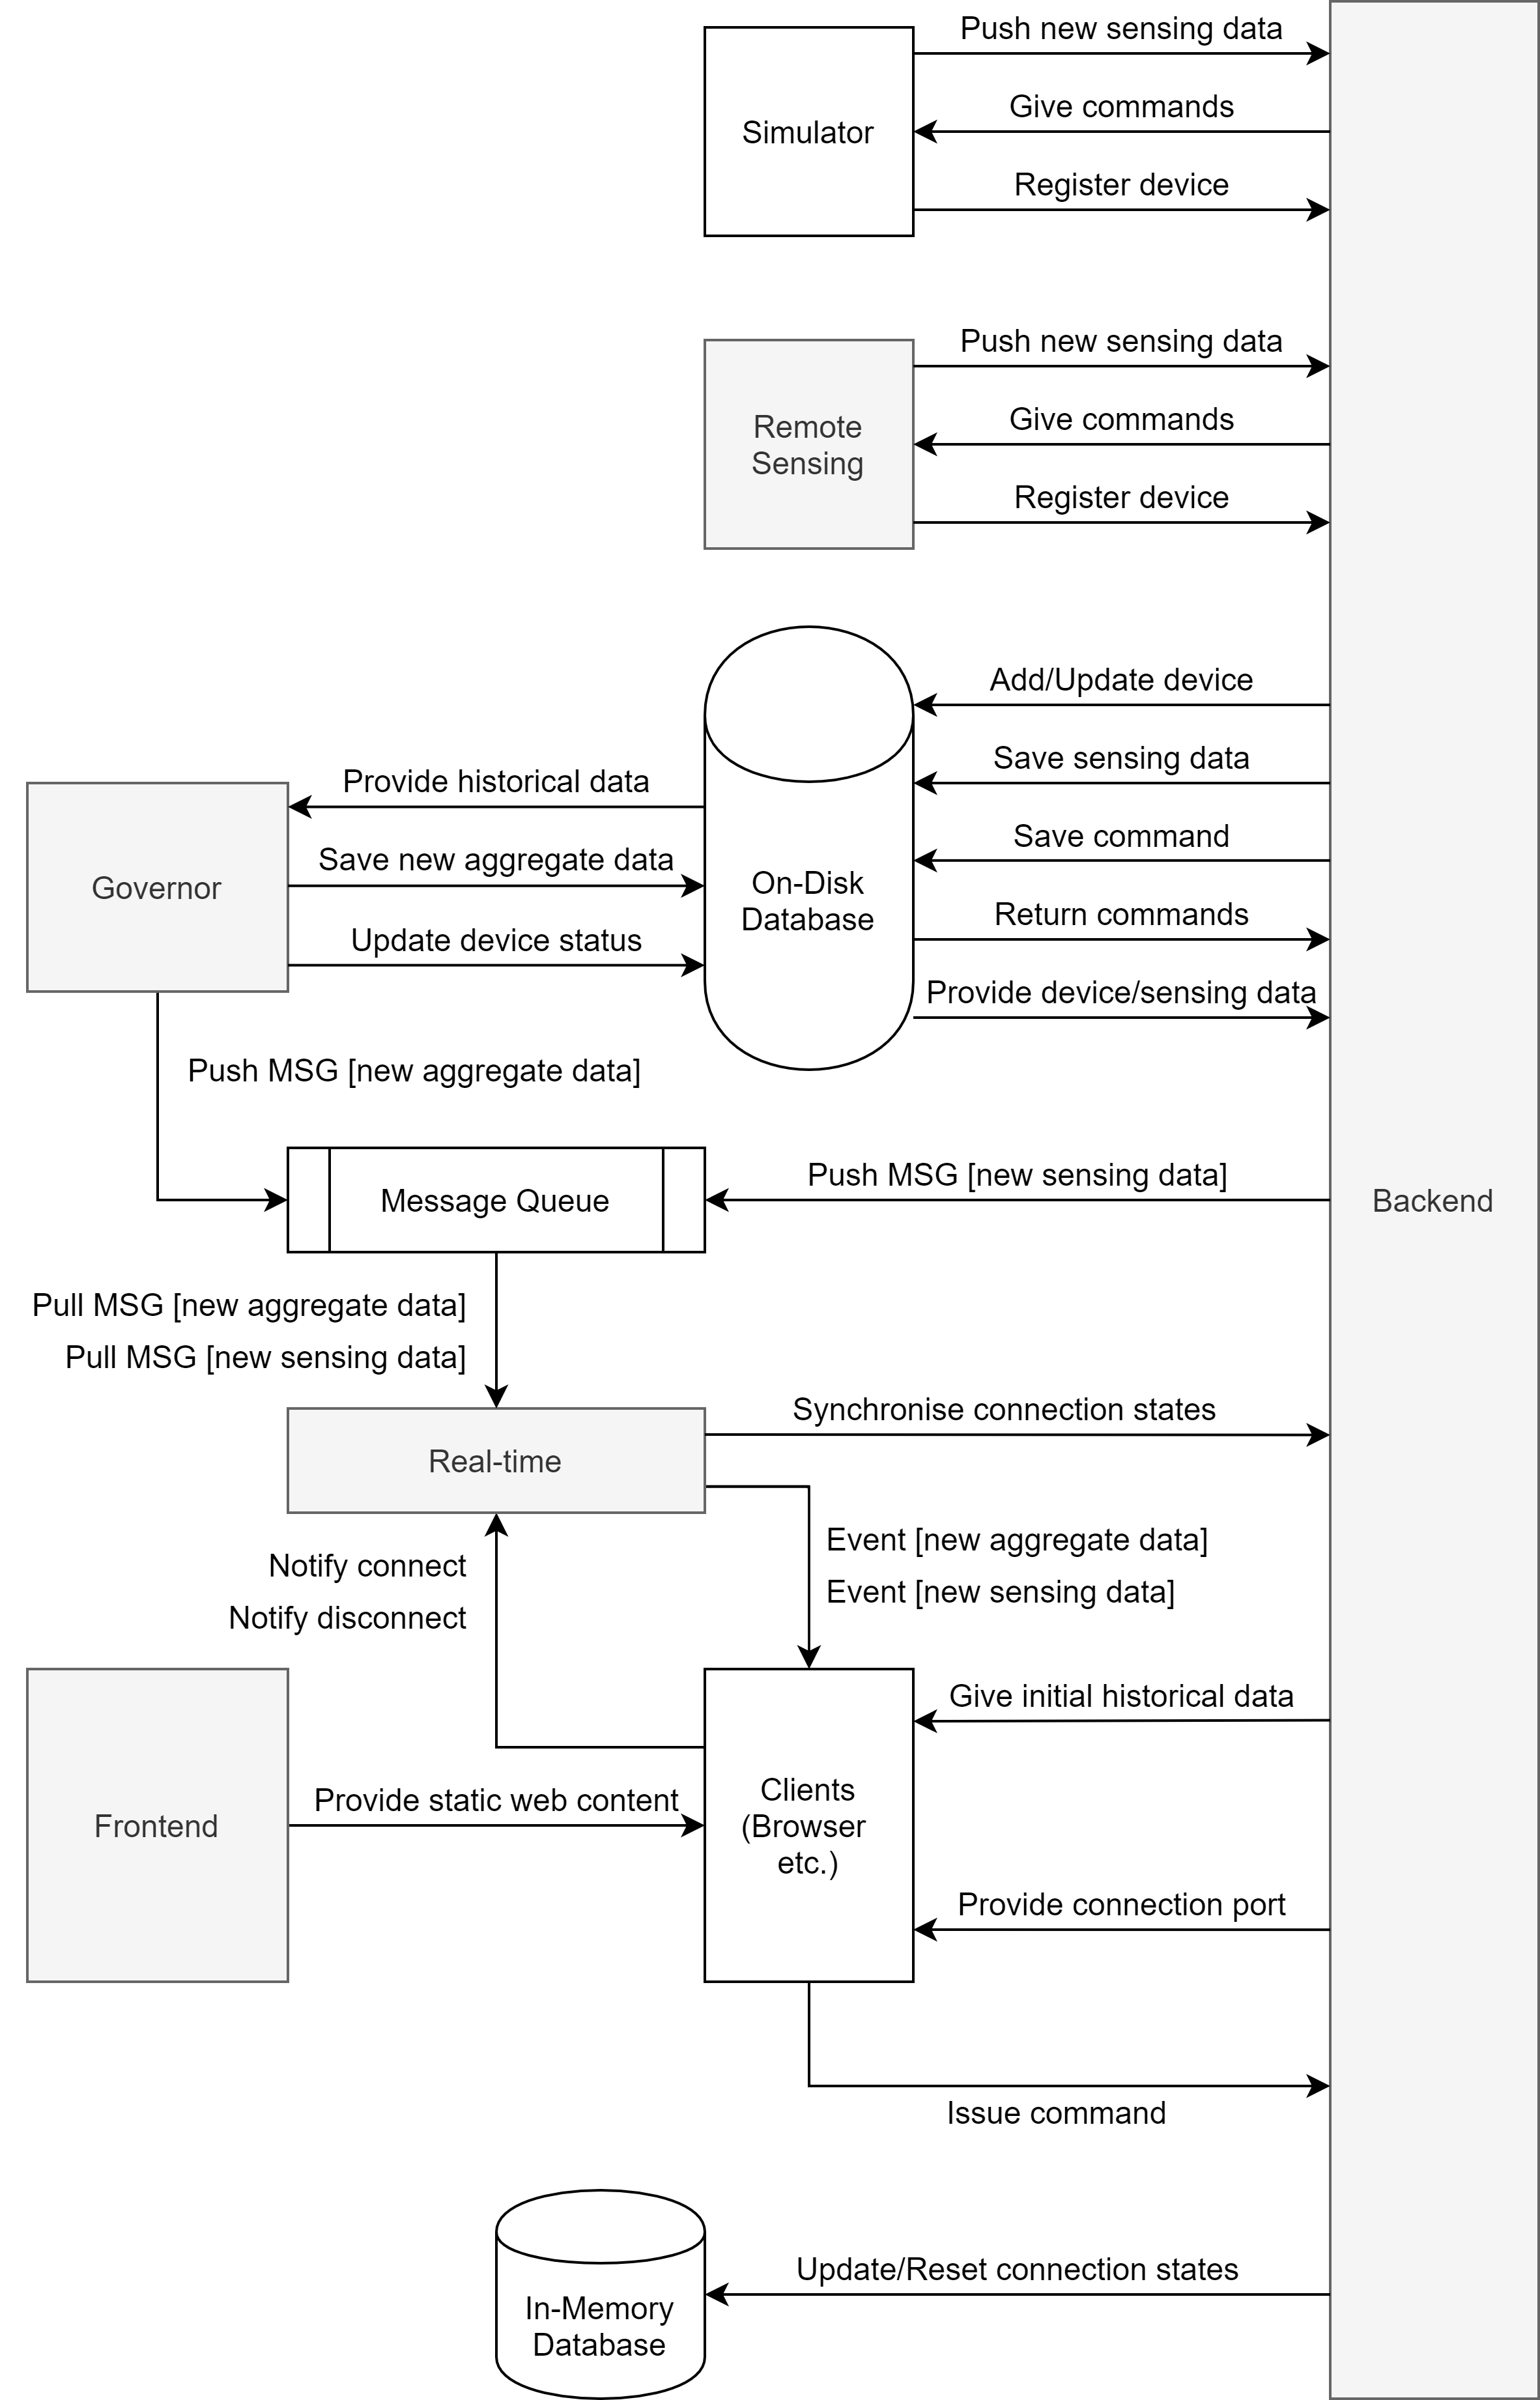
\includegraphics[width=0.82\linewidth]{c4-toplevel.png}
	\caption{Top-level architecture of the proposed system.}
	\label{fig:toplevel}
\end{figure}

\subsection{Initialisation}

The initialisation process is referring to a device in the remote sensing component such as a microcontroller attempting to connect with the server before it can send data and receive commands. When a microcontroller is initialising, it sends a register device request to the backend and then wait for the reply from the backend. Once the request is received by the backend, it tries to find a matching device in the database. If found, then it update the device status to online. Otherwise, it generates a new device ID and create a representation of the new device in the database with status marked as online. Finally, the backend notifies the microcontroller and the intialisation sequence is complete. The figure \ref{fig:init} shows the initialisation process.

The initialisation process achieves two goals, the first one is letting the backend knows the device is online, and the second one is getting a unique ID so that it can be identified in the future. 

\begin{figure}[!ht]
	\centering
	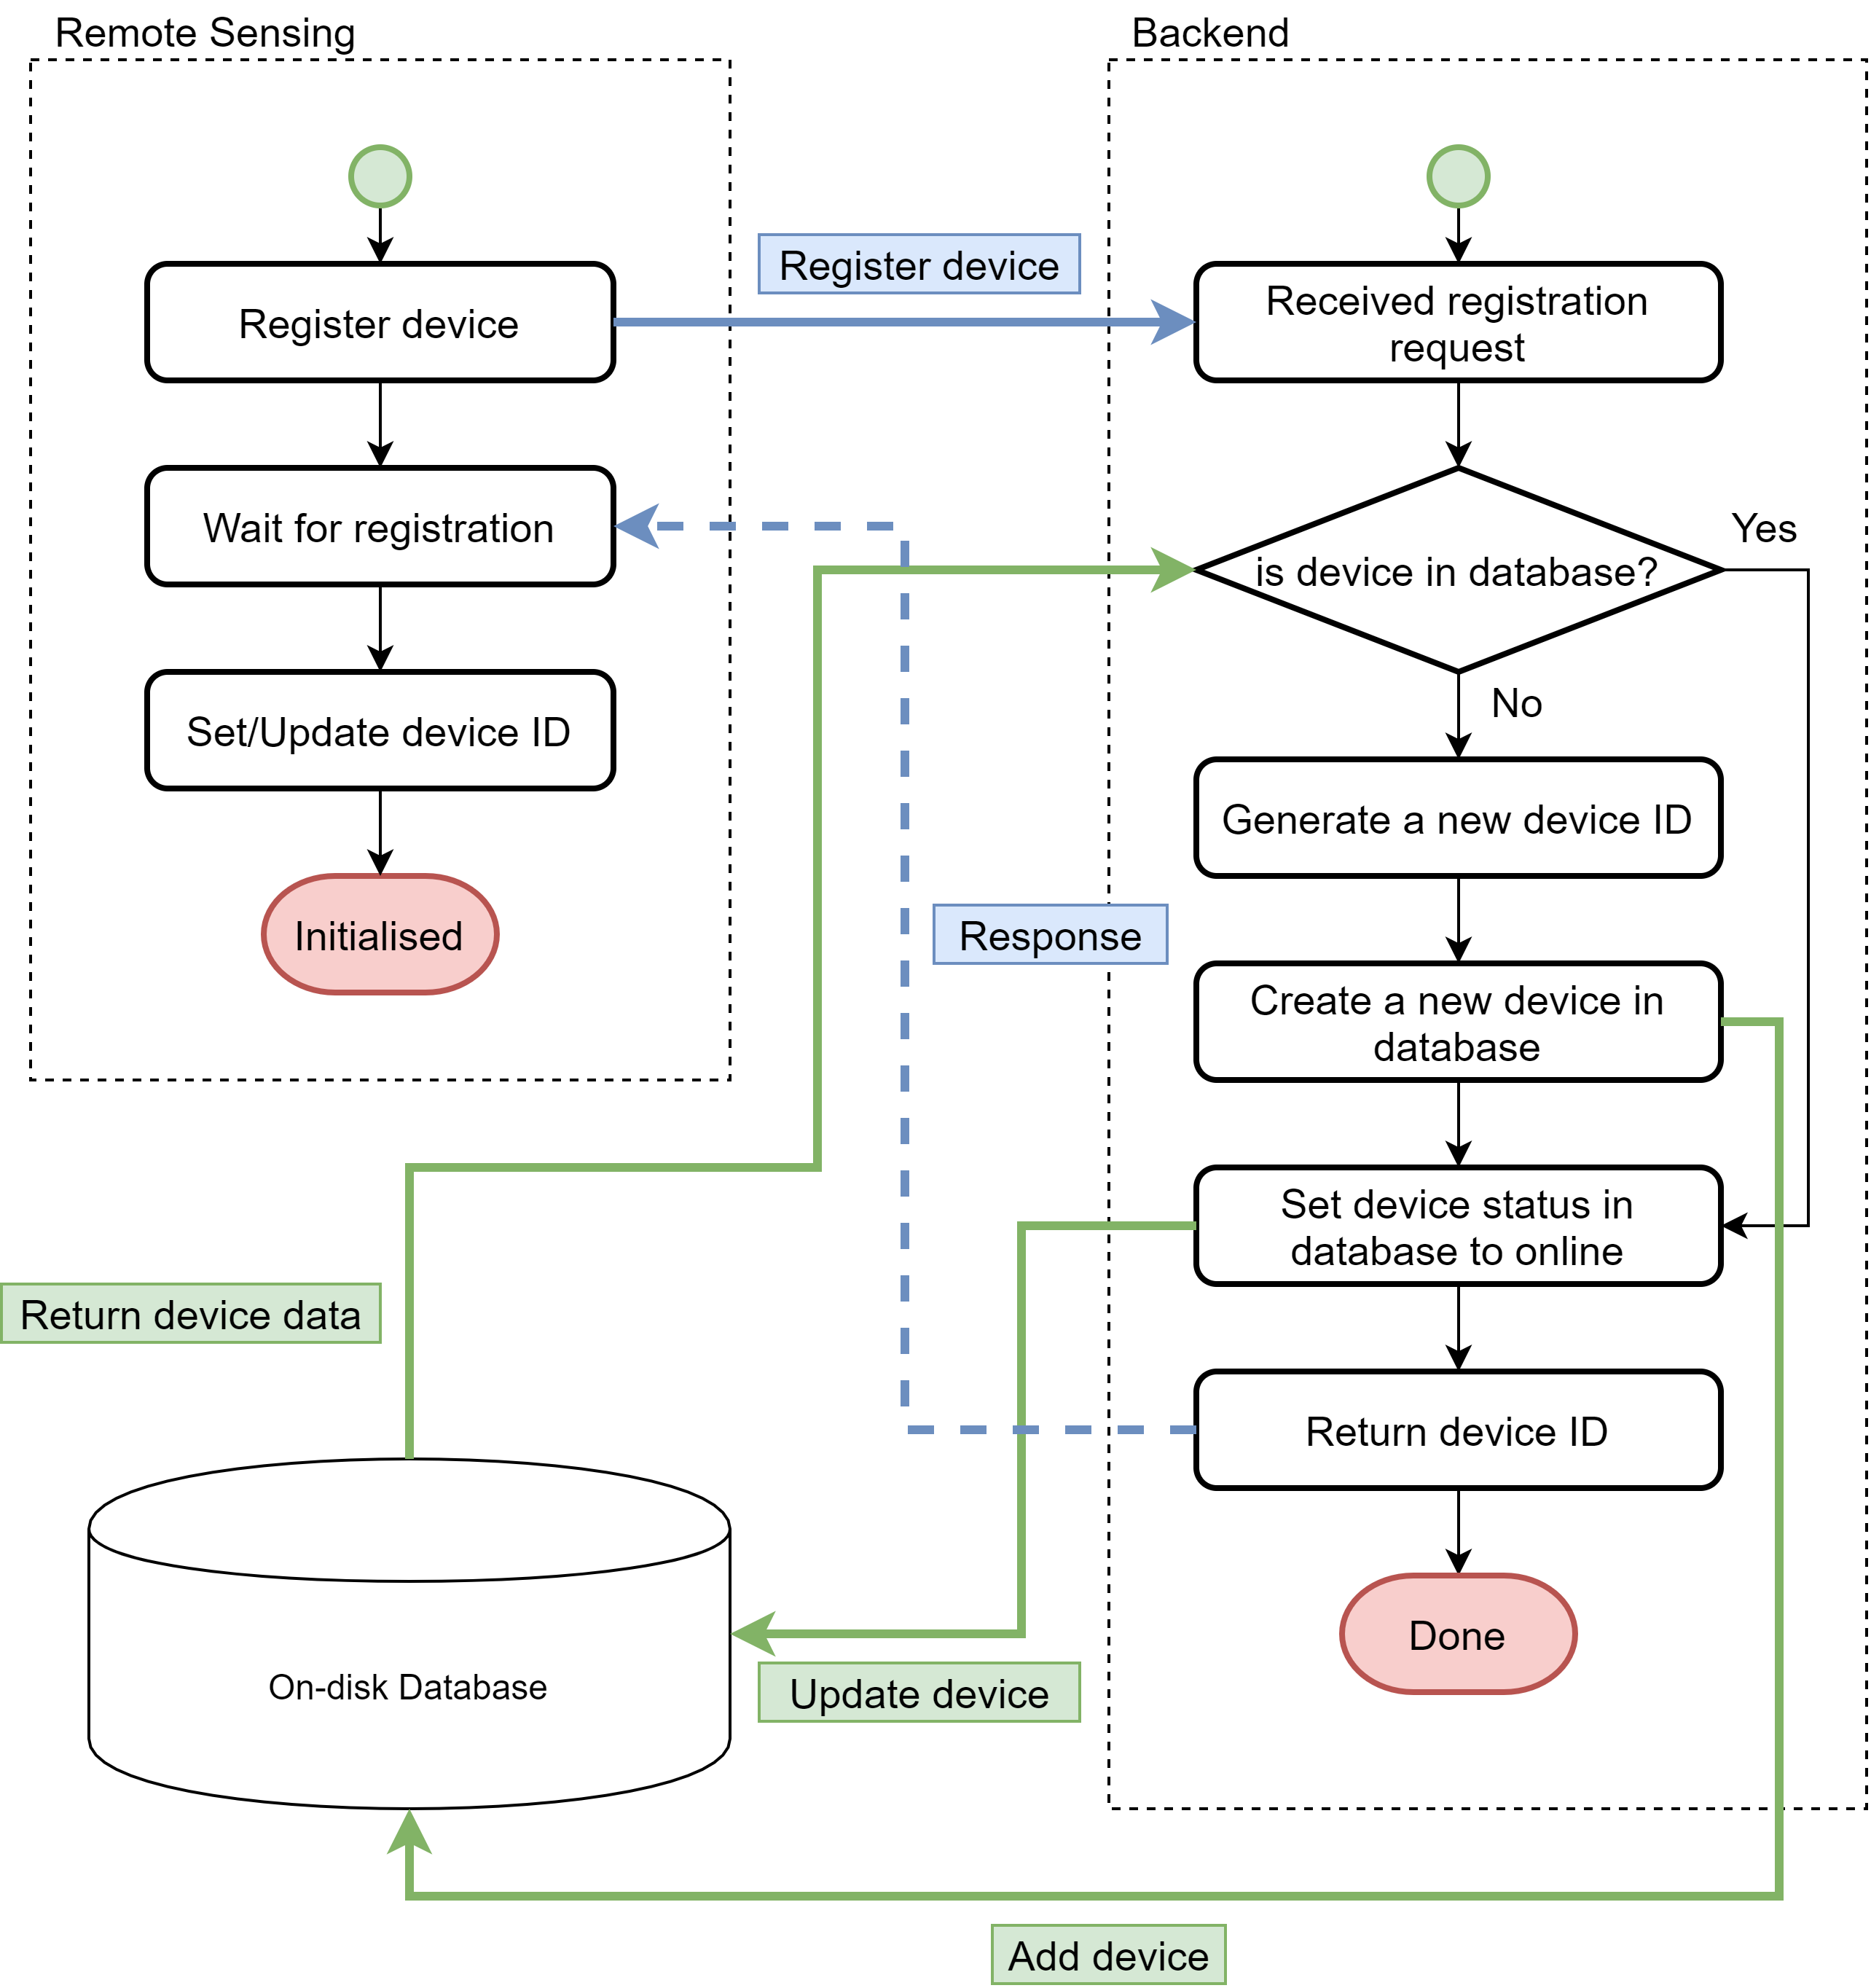
\includegraphics[width=\linewidth]{c4-initialisation.png}
	\caption{The initialisation process.}
	\label{fig:init}
\end{figure}

\newpage


\subsection{Data recording}

The monitoring process starts from recording the data from sensors

\subsection{Data monitoring}


\subsection{Controlling}

\newpage
\section{Remote sensing}
\label{sec:remoteSensing}
sdfsdf

\section{Backend}
\label{sec:backend}
sdfsdf
\section{Frontend}
\label{sec:frontend}
sdfsdf
\section{Real-time}
\label{sec:realtime}
sdfsdf
\section{Governor}
\label{sec:governor}
sdfsdf
\section{Simulator}
\label{sec:simulator}
sdfsdf
\section{Client}
\label{sec:webClient}


\end{document}